% !TEX program = xelatex
\documentclass[article, 12pt, a4paper]{memoir}

\usepackage[UKenglish]{babel}
\usepackage{csquotes, ellipse, longtable}
\babelprovide[hyphenrules=UKenglish]{UKenglish}
\hyphenation{} % Specify hyphenation. Words are divided by spaces.

\usepackage{graphicx}
\usepackage{float}
\usepackage{hyperref}

\usepackage[margin=1in]{geometry}

\usepackage[authordate, backend=biber]{biblatex-chicago}
%\usepackage[backend=biber, style=chicago-authordate]{biblatex}
\addbibresource{$HOME/Documents/ConfigAndTemplates/LaTex/zotero-library.bib}
\SetCiteCommand{\autocite}

\usepackage{amssymb, titling}
\usepackage{enumitem}
\setlist[itemize]{itemsep=.25em}
\setlist[enumerate]{itemsep=0em}

%\usepackage{newtx} % Change font here. Comment out to use Computer Modern.
%\usepackage[T1]{fontenc}

\renewcommand{\chaptitlefont}{\normalfont\Large}
\renewcommand*\thechapter{\arabic{chapter}.\hspace{-10pt}}
\renewcommand*\thesection{\arabic{chapter}.\arabic{section}.\hspace{-8pt}}
\renewcommand*\thesubsection{\arabic{chapter}.\arabic{section}.\arabic{subsection}\hspace{-8pt}}
\setsecheadstyle{\normalfont\large}


%%%%%%%%%%%%%%%%%%%%%%%%%%%%%%%%%%%%%%%%%%%%%%%%%%%%%%%%%%%%

\title{\Huge Empty Hand Basics (v0.1.0)} % Specify title. If using \thetitle, etc. specify fontsize, e.g. \huge
% \thanks{}
\author{\Large Lauge Dideriksen, \today} % As with title, although \Large seems to work well.
\date{}

%%%%%%%%%%%%%%%%%%%%%%%%%%%%%%%%%%%%%%%%%%%%%%%%%%%%%%%%%%%%

\begin{document}
%\pagenumbering{gobble} % Removes page number. Nice for single page documents.
\OnehalfSpacing

% TITLE VERSION I
%\pretitle{\vspace{-30pt}\HUGE\begin{flushleft}}
%\posttitle{\par\end{flushleft}}
%\preauthor{\vspace{-20pt}\begin{flushright}}%figure out how to make flush with title.
%\postauthor{\par\end{flushright}\vspace{-50pt}}
%\maketitle
%\noindent\parbox[t][][t]{\linewidth}{%
	%\parbox[t][][t]{.6\linewidth}{\thetitle}
	%\hfill%
	%\parbox[t][][t]{.4\linewidth}{\raggedleft\theauthor}
%}

% TITLE VERSION 2
{\raggedright\thetitle}\medbreak	
{\raggedright\theauthor}\bigbreak

% TITLE VERSION 3
%\maketitle

\captionnamefont{\footnotesize}\captiontitlefont{\footnotesize}
\begingroup\let\clearpage\relax\raggedbottom


%%%%%%%%%%%%%%%%%%%%%%%%%%%%%%%%%%%%%%%%%%%%%%%%%%%%%%%%%%%%%%
% WRITE BELOW
%%%%%%%%%%%%%%%%%%%%%%%%%%%%%%%%%%%%%%%%%%%%%%%%%%%%%%%%%%%%%%

\noindent This document is an attempt at a curriculum covering the basic use of the empty hand\footnote{Througout this document, I use the term `empty hand', instead of `off hand' or similar. I do so to emphasise it as an essential component of fencing with the rapier `alone', rather than an unfortunate byproduct of human physiology.} in Italian rapier fencing.
There are three sections: principles, knife work, and rapier work.
The first section sets out the principles which the remainder of the document attempts to put into practice.
The second sections contains a collection of drills and free play excercises to be done with training knives.
This is not an attempt at a knife fighting curriculum, but a way of teaching and practicing mechanics and movement patterns without the added complexity of maneouvering a 110cm length of steel.
The third section contains drills and free play exercises focused on using the empty hand with the rapier.
It also contains a collection of plays from various primary sources that use the empty hand.

\section*{How To Use this Document}
Each section of this document builds on the previous: the principles laid out in section one lay the foundation for the mechanics and movements in section two on knife work.
The second section contains drills and exercises to familiarise the student with using the empty hand.
Once those mechanics have become familiar, the third section combines them with the blade- and footwork of Italian rapier fencing.
Finally, the plays at the end of the third section integrate the empty hand as part of longer sequences.
Each drill is focused on a single technique and several drills can be combined to form decision drills.
The free play exercises are meant to be a transition between drilling and sparring; they are constrained and often asymetrical, but should be carried out with increasing intensity.

In an ideal world, the sections should be covered in order over the course of several weeks.
That, however, is hardly viable when teaching a rapier class in a fencing club.
The next best thing is to pick out a combination of knife and rapier drills and exercises covering the same topic, and use that as the basis for a class.
Even so, I would advice against introducing the primary source plays before the class has a good grip of the fundamentals.

\section*{A Note for (and against) Left-handed Fencers}
As always, drills and excercises need to be adapted when fencing (against) an opponent who wields their weapon in a different hand than you do.
For most drills in this document, it should suffice to switch the side of attack (inside/outside), but in cases where it is not, I have made a note suggesting how to modify it.
Even so, there might be exercises that are simply not appropriate when fencing `leftie' against `rightie'.
In those cases, trying to force an a technique to work is a waste of time, and the better solution is for the fencer on the `receiving end' to fence with their other hand.

\section*{Terminology}
Broadly speaking, there are four ways to use the empty hand in Italian rapier fencing: parrying, taking over, trapping, and displacing.\footnote{Fencing terminology is infamously inconsistent and this topic is no exception. These are the terms I have settled on.}
In an empty-hand parry, the opponent's weapon is deflected first, and usually only, with the empty hand.
This is often combined with a simultaneous (\emph{stesso tempo}) attack with the rapier.
As a rule of thumb, empty-hand parries do not work against cuts.\footnote{They can, but it is a bit sketchy. See e.g. Di Grassi's \citetitle{digrasssiHisTrueArte2000}.}
When the opponent's blade is parried or displaced with the rapier, the empty hand can take over controlling their weapon, freeing up the rapier for offensive use.
Trapping is any form of taking control over the opponent's weapon.
This ranges from the complex traps and disarms found in some Spanish sources to simply grabbing any part of the opponent's weapon within reach.\footnote{Oppinions differ on whether it is possible to hold on to a sharpened rapier or not; to my knowledge, it has been some time since anyone tried it out.}
Finally, the empty hand can be used to displace the opponent's blade and create an opening (similarly to a \textsc{battuta}).

While there are examples of all four types of empty-hand actions in Italian rapier treatises from the seventeenth and eighteenth centuries, parrying and taking over are by far the most common.
For that reason, they are the focus of this document.
Although it seems like an obvious thing to do, I am not aware of treatise describing the offensive use of the empty hand in the form of punching, slapping, eye-poking, etc.
Whether that accurately reflects how people fenced at the time is another matter altogether.

\chapter{Principles}

It seems to me that there are three fundamental principles for successfully integrating the empty hand with the rapier:
\begin{enumerate}
    \item The empty hand must not get in the way of the rapier.
    \item The empty hand must be ready to use without any preparatory movement.
    \item The empty hand must be an intentional part of every action.
\end{enumerate}
These three principles are in addition to the general principles of fencing in general and rapier fencing in particular.

From (1.) it follows that the empty hand is most easily used on the inside.
On the inside, any thrusting attack to the head and torso can be deflected with the same movement of the empty hand: a semicircle from just above the head to somewhere outside the left hip.
Using the same motion to cover the entire inside also means that the movement removes a decision point, as opposed to holding the empty hand in the middle and moving it up or down depending on the opponent's target.
Doing this motion from the top down rather than the bottom up means that gravity works with you and against your opponent.
Depending on context, it can be useful to `tilt' this imaginary semicircle towards the opponent, by moving the end point forward and upward.
In this way, the parrying movement can also be used to displace and to take over when the opponent's blade is on the inside.

From this in combination with (2.), it follows that, in the guard, the empty hand should be held somewhere around head-height and close to the face.
Assuming a \emph{capoferrian} guard, the body must be angled so that the empty hand can protect both face and torso without having to turn the torso first.
Exactly what this looks like will vary from fencer to fencer.

Parrying, displacing, and taking over on the outside come with some downsides, but should nonetheless be part of one's repertoire.
The most obvious downside is that they require crossing the arms, thus necessarily limiting the weapon arm's movement upward or downward.
Another downside is that they require more precision.
Using the sweeping motion described above, actions on the inside have a wide margin of error---a parry will work whether one catches the opponent's blade with the hand, wrist, or forearm.
Such a motion is not practical on the outside, instead actions on the outside tend to be horizontal.
At the same time, most rapier schools use a guard where the outside is `closed'.
Attacks on the outside therefore tend to follow from invitations, \textsc{battuti} or feints.
By drilling responses to these that incorporate the empty hand, one can alleviate some of those downsides.

\bigbreak
So much for platonic fencing.
These are principles, not commandments and they will not apply to every situation.\footnote{Such as your opponent's avoiding your empty-hand parry by lifting their tip over your hand, as is suggested in \emph{Den Ridderlige og Adelige Fecht-konstis} (\citeyear{a.RidderligeOcAdelige1646}). Any empty-hand action immediately following that will likely start from below, as that is where the hand is.}
Nonetheless, this document is concerned with the basics, and for that these principles will apply nine times out of ten.

\chapter{Knife Work}
As I wrote in the introduction, this section does not describe a system of knife fighting.
Many of the drills and patterns are taken from or inspired by various knife systems, but the goal here is to get used to using both hands in concert, not to become proficient at using a knife.
Working with knives when learning to use the empty hand has several advantages.
For one, knives are much shorter and much lighter than rapiers.
This makes the discrepancy between the hands is smaller.
The lighter weight also allows more repetitions of new movements before fatigue becomes an issue.
The most important distinction between knife work and rapier fencing, however, is that knife fighting is not fencing---there is no fancy footwork, no seventeenth-century flair.

Not all knives are created equal and the same goes for training knives, but each different implement affords different ways of training.
I make the people in my class work with all of them---plastic bowies, LARP daggers, aluminium trainers, rolled-up newspapers, etc.
A trainer I find especially useful for higher-intensity work is a {\char`\~16cm} roll of yoga mat, two-thirds of which is wrapped in gaffer's tape to form a handle.\footnote{I have taken this idea from Scott Babb's knife fighting system, \emph{Libre}.}
It is cheap, stiff enough to be usable, yet soft enough that neither student nor teacher need to worry about anyone getting hurt.

As for posture, grip, and footwork: keep it simple.
Feet shoulder-width apart, weight on the balls of your feet, slight bend in the knees, shoulders almost square to the opponent/partner, posture relatively upright, weapon slightly in front of the body but not too far, and empty hand has described above.\footnote{This is intentionally vague. Find something that allows you to move well and is dinstinctly different from your rapier guard. Don't overthink it.}
Hold the weapon point down or point up (hammer or sabre grip to suit preference and implement) depending on exercise and do not lock the wrist.
In terms of footwork, think boxing or Philippino triangle footwork, not fencing.
And whatever you do, do not lunge!

\section{Drills}
\subsubsection*{Dui Tempi}
\begin{enumerate}
    \item Implement: larger blade, e.g. bowie held point up.

        A attacks with a diagonal cut to the head (number `1' or `2').
        
        B blocks with a cut to the forearm, takes over the parry with the empty hand, and strikes A with a cut or a thrust.
        
        \textbf{Note}: experiment with different placements of the empty hand in relation to the blade.
    \item As above, but A attacks with a thrust to the face or chest.
    \item Implement: smaller blade, preferably held point down.

        A attacks with a diagonal thrust to the outside of B's neck.

        B blocks with the forearm of their weapon hand.

        A clears the block out of the way (downwards) and finishes the attack.

        \textbf{Note}: this drill and the following does not work R against L.

    \item As above, but B blocks with their empty hand.

        A clears the parry again, this time more sidewards than downwards.

        \textbf{Flow}: this drill can be combined with number 3 into a flow/reaction drill.
        Depending on B's block, A will have to clear differently.
        B can also block first with the weapon hand and then with their empty hand, forcing A to clear twice.
    \item As 3 and 4 above, but A's attack is aimed at the inside of B's neck.

        \textbf{Flow}: These two can be combined with 3 and 4 to create a flow drill where both A and B have to react to each other.
    \item Implement: smaller blade, held point down.

        A attacks with a forehand to B's face/neck.

        B blocks with the forearm of their empty hand, seeking to counter (\emph{in due tempi}) to A's trunk.

        A rips down through B's block, while either checking their weapons shoulder or delivering a palm strike to their face.

        \textbf{Note}: This drill is not suitable leftie against rightie.

\end{enumerate}

\subsubsection*{Stesso Tempo}
\begin{enumerate}
    \item Implement: blade of any size, held point up or point down.

        A attacks with a diagonal cut to the head (number `1' or `2').

        B steps toward A while simultaneously blocking the attack with the empty hand and striking A with a cut or thrust.

        \textbf{Note}: try out different forms of empty-hand blocks---hand, forearm, trapping, or the kind of elbow `crash' found in systems like \emph{UC} and \emph{SPEAR}.
    \item Implement: blade of any size, held point up or point down.

        A attacks with a thrust to the trunk.

        B parries with their empty hand while striking A with a cut or a thrust.

    \item Implement: blade of any size, held point up or point down.

        A attacks with a horizontal cut/thrust to the outside face or neck.

        B steps in, thrusting A in the chest while moving the empty hand across to the outside of their face, checking A's arm/elbow.
\end{enumerate}

\subsubsection*{Free Play}
%TODO: Add general description. Include notes on distance, speed, pressure, etc.
\begin{enumerate}
    \item A fights as usual, but B cannot use their empty hand.
    \item As above, but B is up against a wall.
    \item As above, but it is A against the wall.
    \item Both can use the empty hand, but one is against the wall.
    \item Fight as usual, but in a confined space.
    \item Limited targeting: the only valid targets are e.g. the back, the face, or the trunk.
    \item Multiple hits: Do not reset after each hit, but continue until someone has been hit multiple times.
    \item As above, but pursue a situation where the opponent is unable to counter, even if given tempo to do so.
\end{enumerate}


\chapter{Rapier Work}
%TODO: Add description
Before attempting any of the drills below, spend some time integrating the lessons learned from the knife work into your rapier basics---especially stance and footwork.
Look for the feeling of symmetry between weapon hand and empty hand that has hopefully developed with the knife.

The following drills differ in some ways from the plays traditionally found in rapier treatises.
They are short.
Few have more than three steps.
This is to keep the focus on the technique of movement being drilled.
I have also tried to emphasise offensive actions, as the treatises tend to emphasise defensive ones.
Much like primary source plays, however, not every drill is likely to work in sparring, and not every drill will work for every fencer.


\section{Drills}
\subsubsection*{Dui Tempi}
\begin{enumerate}
    \item A attacks with a diagonal cut to the head (number `1' or `2').
        
        B parries in \textsc{quarta} or \textsc{secunda}, depending on the attack, takes over the parry with the empty hand, and strikes A with a cut or a thrust.
        
        \textbf{Note}: experiment with different placements of the empty hand in relation to the blade.
    \item As above, but A attacks with a thrust to the face or chest.
    \item As above, but A attacks with an inside thrust to the abdomen, and B parries in hanging \textsc{prima} or low \textsc{quarta}.
    \item A attacks with a thrust to the abdomen in \textsc{terza} or \textsc{secunda}.

        B parries with a hanging \textsc{secunda} to their outside, steps forward with a \textsc{passata}/Profilwechsel, grips the hilt or base of A's blade, and simultaneously pulls with their empty hand while thrusting with the rapier under A's blade.
        Ideally, A's blade should be trapped between B's empty hand and their quillons.

        \textbf{Note}: depending on the length of the rapier, it may be necessary to keep the weapon hand relatively far back during the \textsc{passata}.

        \textbf{Variation 1}: instead of thrusting with the point, B can keep their rapier point-down and hit A in the face with the hilt.
        This is particularly nasty if the rapier has straight quillons.
    \item As above, but instead of levering A's blade between empty hand and own quillons, B frees their blade, lifts their arm behind them, and thrust A from above.
    \item As above, but instead of gripping A's blade, B pushes the elbow of A's weapon arm.\footnote{Cf. the Fiore de'i Liberi adaptation below.} This is especially effective if the rapier parry has the force  of a \textsc{battuta}.
    \item A attacks on the inside with a diagonal cut to the head or shoulder.

        B parries with a hanging parry (\textsc{octav}), steps forward with the back leg and grips A's forearm with their empty hand. Riposte at will.

    \item Same as above, but A attacks on the outside and B parries accordingly (\textsc{septim}).
\end{enumerate}

\subsubsection*{Stesso Tempo}
\begin{enumerate}
    \item A engages B with \textsc{stringere} on the inside, seeking to close the distance.

        As soon as B's point comes within reach, A simultaneously clears it out of the way and thrusts B in \textsc{quarta}.

        \textbf{Note}: `had B been a shrewd person' they would have never let A get that close. Well, B isn't always shrewd.

    \item A engages B with \textsc{stringere} on the outside, seeking to provoke a disengage.

        B disengages to the inside when they feel forced to do so.

        As soon as B disengages, A advances or lunges, while simultaneously clearing B's rapier with the empty hand and thrusting B in \textsc{quarta} or \textsc{secunda} (see note).

        \textbf{Note}: Depending on how early B disengages, A's timing will change drastically.
        Making the final thrust in \textsc{quarta} will provide A with more protection, while thrusting in \textsc{secunda} will leave slightly more space for the empty hand to work.

    \item As above, but B thrusts in opposition directly following their disengage.
        
        As A parries and thrusts, they can either stand their ground or step to their inside with a traverso.\footnote{Yes, this is towards, not away from, the incoming attack. The idea is to further displace the opponents blade, while keeping it under control.}
\end{enumerate}

\subsubsection*{Free Play}
\begin{enumerate}
    \item A fence as usual, but B cannot use their empty hand.
    \item As above, but B is up against a wall.
    \item As above, but it is A against the wall.
    \item Both fencers can use their empty hand, but one has their back against the wall.
    \item Multiple hits: Do not reset after each hit, but continue for until someone has been hit multiple times.
    \item As above, but pursue a situation where the opponent is unable to counter, even if given tempo to do so.
\end{enumerate}

\section{Primary Source Plays}
The following plays have been taken from a variety of rapier treatises.
Where the author gives several responses to an action, only those using the empty hand have been included.
For the sake of brevity, I have rewritten them in a more schematic form, but I highly recommend consulting the original sources, or translations thereof.

\citeauthor{wilsonRidolfoCapoFerro2025} plays are based on Wilson and Swanger's translation.
Plays from \citeauthor{fabrisSalvatorFabrisWiktenauer}' treatise are based on Michael Chidester's transcription of A. F. Johnson's translation.
The \citetitle{FioreLiberiSword} play is based on translations by Michael Chidester and Colin Hatcher
Both are available on \href{https://wiktenauer.com}{Wiktenauer}.
Plays from \emph{Den Ridderlige oc Adelige Fechtkonstis grundelige oc Methodiske Beskriffuelse} are based on my own translation.

\subsubsection*{Capo Ferro No. 20}

\begin{figure}[H]
    \begin{center}
        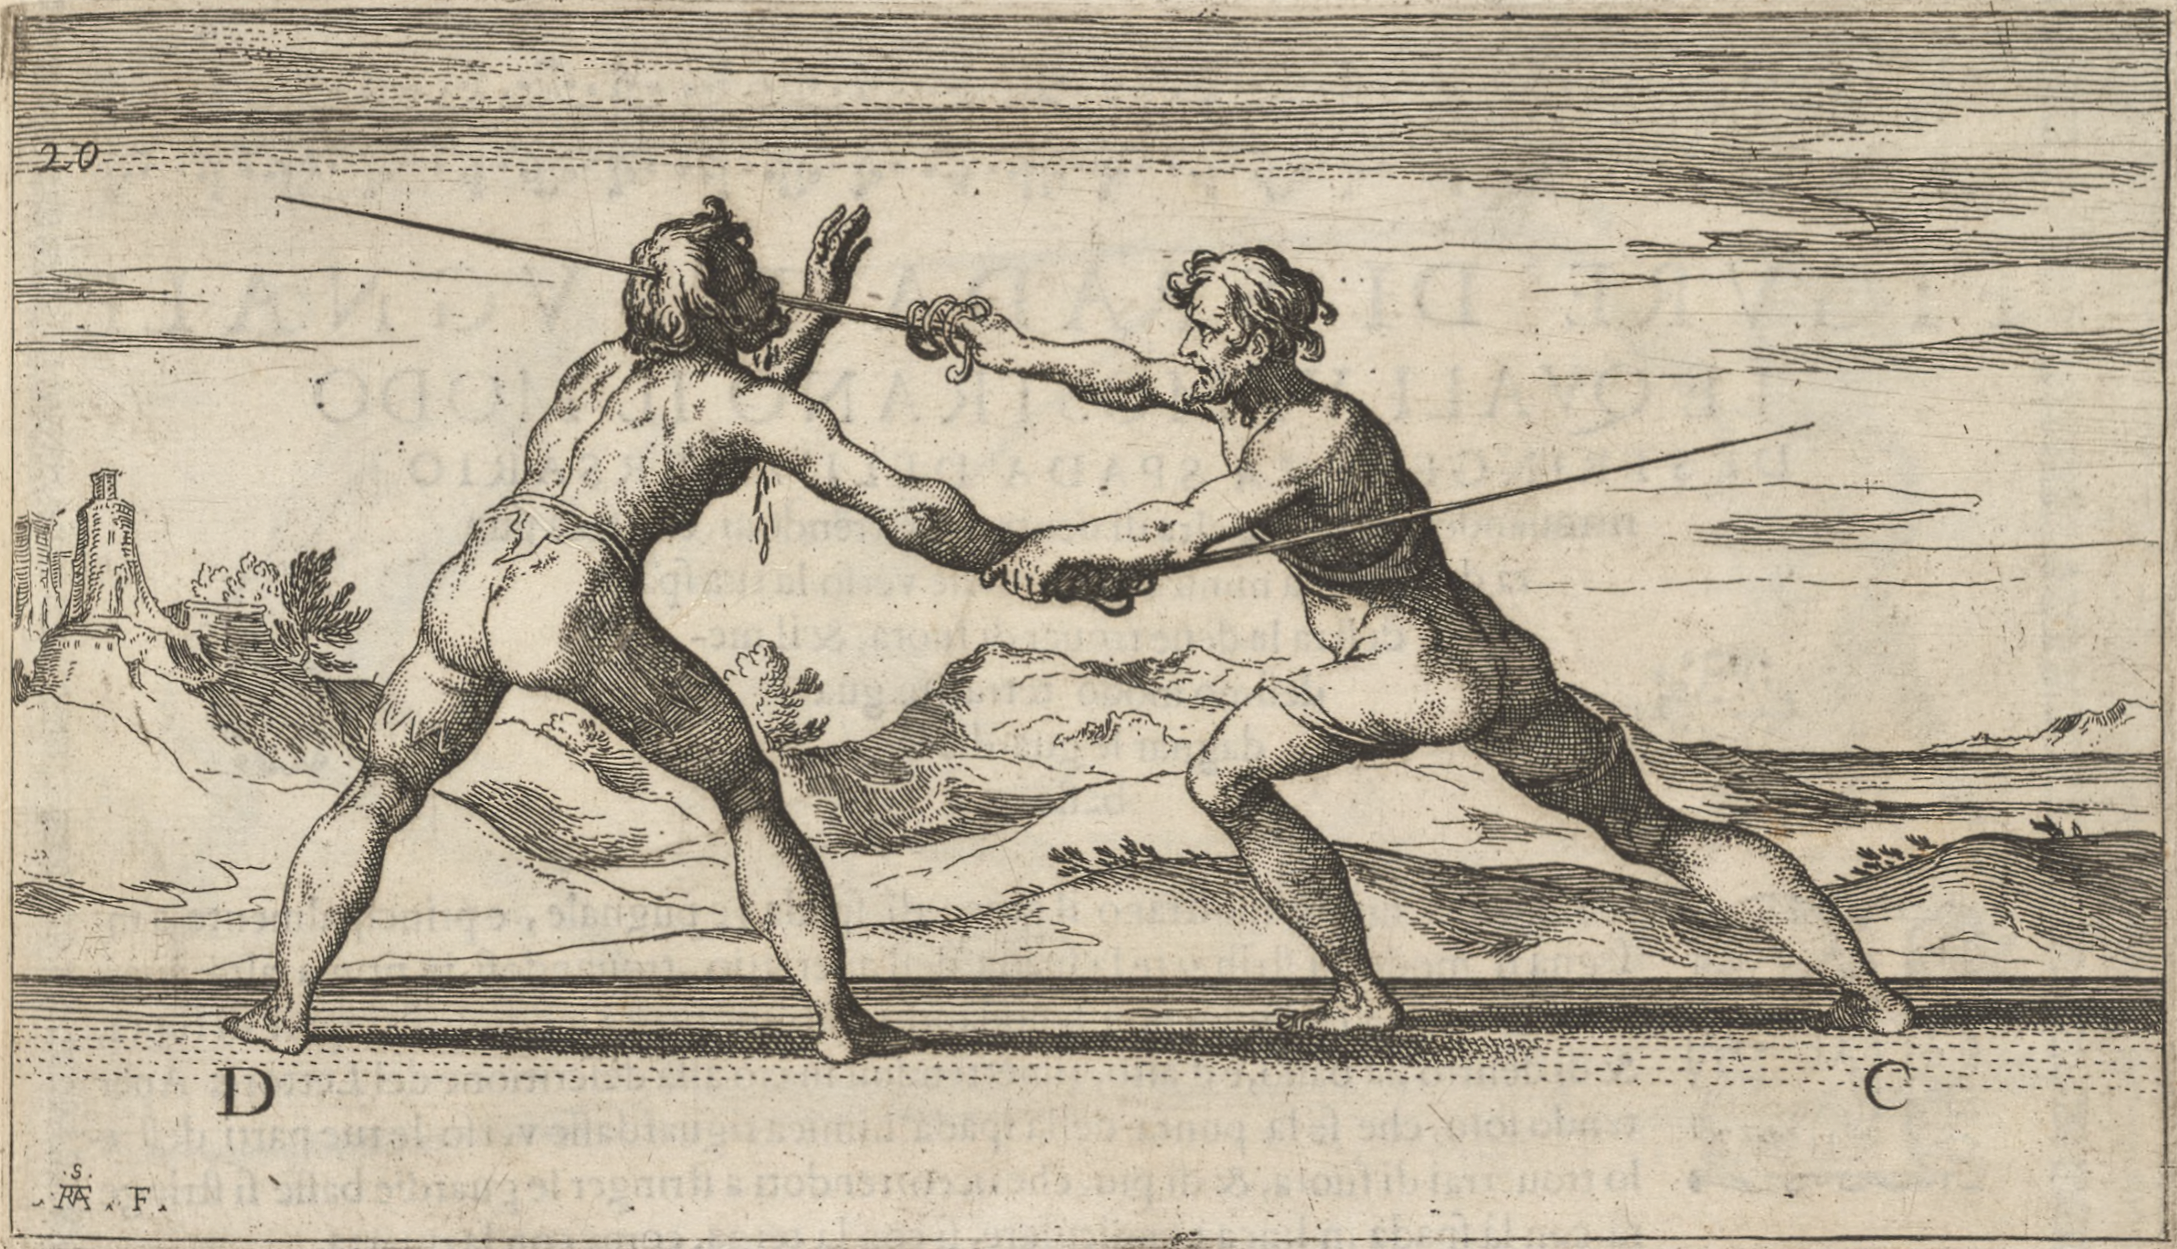
\includegraphics[width=0.95\textwidth]{./Capo_Ferro_20.png}
    \end{center}
    \caption{\protect\url{https://wiktenauer.com/wiki/File:Capo_Ferro_20.png}}
\end{figure}

C \textsc{stringere} D on the outside.

D disengages, seeking to strike C with a \textsc{stoccata}.

\textbf{Option 1}: C parries in \textsc{quarta} with a beat of the front foot.\footnote{I take this to mean an \emph{appell}, but also a transfer of weight to the front foot.}
C then strikes D's face in \textsc{seconda} with a \textsc{passata}, while gripping D's wrist with the empty hand from above.

\textbf{Option 2}: C parries in \textsc{quarta} while closing with the back foot.
C then strikes D's face in \textsc{seconda} with a lunge, while gripping D's wrist with the empty hand from above.

\subsubsection*{Fiore de'i Liberi}

\emph{Fiore de'i Liberi} is a treatise from before rapiers were a thing and, as such, the fencing it describes differs somewhat in style from Italian rapier treatises.
This technique still works, however, especially for more athletic fencers.
I have included it here as an example of a more forceful use of the empty hand.

\begin{figure}[H]
    \begin{center}
        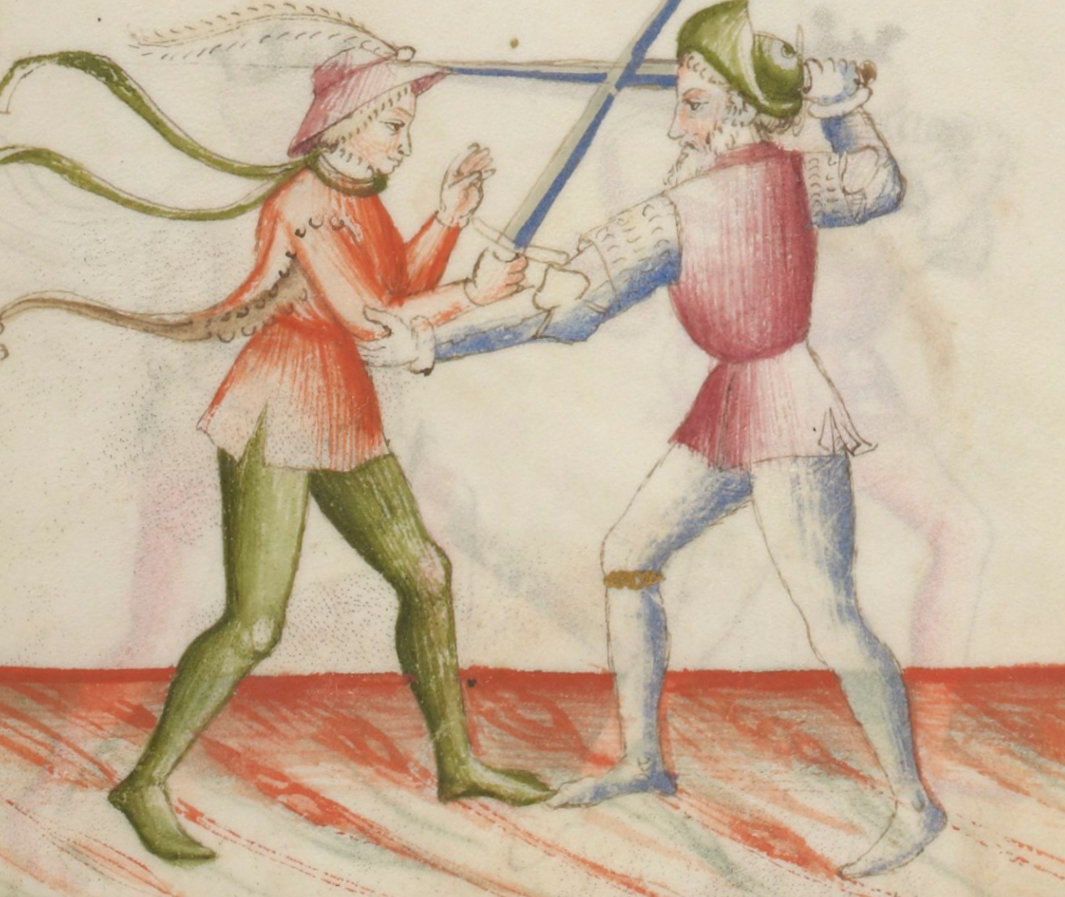
\includegraphics[width=0.95\textwidth]{./MS_Latin_11269_12r-d.png}
    \end{center}
    \caption{\protect\url{https://wiktenauer.com/wiki/File:MS_Latin_11269_12r-d.png}}
\end{figure}

A attacks B on the inside with a thrust in \textsc{prima} or \textsc{secunda}.

B parries in \textsc{quarta}.

As B parries, A steps forward with a \textsc{passata} and shoves B's elbow across their body.

B then `wrap[s his] sword around [A's] neck from behind, and [A] will have no defense to this.'

\textbf{Note 1}: Several notes on this.
A's initial thrust can either be direct or somewhat diagonal, thus forcing B to parry further out than otherwise.

\textbf{Note 2}: I am aware of two illustrated versions of \emph{Fiore de'i Liberi}.
In one, A is depicted with the right foot in front, in the other with the left foot in front.
Especially with long rapiers, I have found that a \textsc{passata} works better than a lunge.

%BIBLIOGRAPHY
    \SingleSpacing
        \AtNextBibliography{\footnotesize}
        \setlength\bibitemsep{0.5\itemsep}
        \printbibliography

\appendix
\renewcommand\thechapter{Appendix \Alph{chapter}:}
\OnehalfSpacing
\chapter{Lesson Plan Summer 2026}

\section*{Class 1: Taking Over}

\section*{Class 2: Displacing}

\section*{Class 3: Parrying}

\section*{Class 4: Review and a Few Dirty Tricks}

\section*{Class 5: Primary Source Plays}
\endgroup
\end{document}
